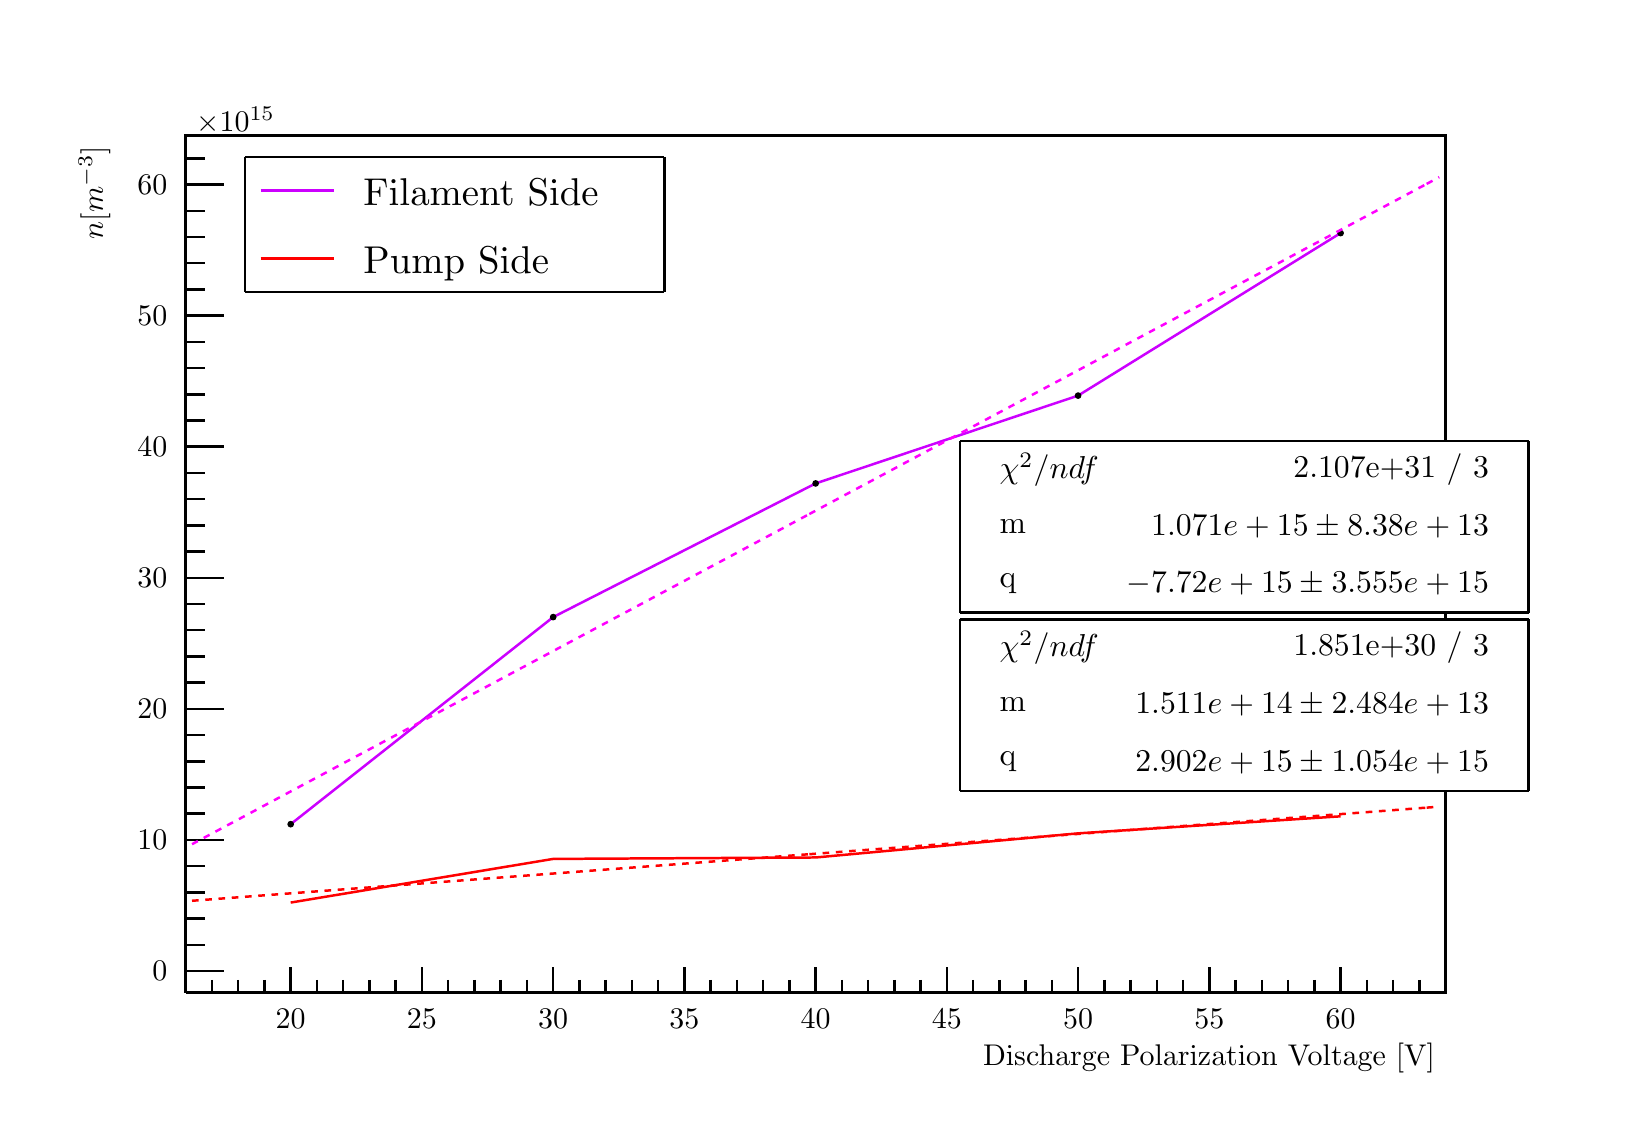
\begin{tikzpicture}
\pgfdeclareplotmark{cross} {
\pgfpathmoveto{\pgfpoint{-0.3\pgfplotmarksize}{\pgfplotmarksize}}
\pgfpathlineto{\pgfpoint{+0.3\pgfplotmarksize}{\pgfplotmarksize}}
\pgfpathlineto{\pgfpoint{+0.3\pgfplotmarksize}{0.3\pgfplotmarksize}}
\pgfpathlineto{\pgfpoint{+1\pgfplotmarksize}{0.3\pgfplotmarksize}}
\pgfpathlineto{\pgfpoint{+1\pgfplotmarksize}{-0.3\pgfplotmarksize}}
\pgfpathlineto{\pgfpoint{+0.3\pgfplotmarksize}{-0.3\pgfplotmarksize}}
\pgfpathlineto{\pgfpoint{+0.3\pgfplotmarksize}{-1.\pgfplotmarksize}}
\pgfpathlineto{\pgfpoint{-0.3\pgfplotmarksize}{-1.\pgfplotmarksize}}
\pgfpathlineto{\pgfpoint{-0.3\pgfplotmarksize}{-0.3\pgfplotmarksize}}
\pgfpathlineto{\pgfpoint{-1.\pgfplotmarksize}{-0.3\pgfplotmarksize}}
\pgfpathlineto{\pgfpoint{-1.\pgfplotmarksize}{0.3\pgfplotmarksize}}
\pgfpathlineto{\pgfpoint{-0.3\pgfplotmarksize}{0.3\pgfplotmarksize}}
\pgfpathclose
\pgfusepathqstroke
}
\pgfdeclareplotmark{cross*} {
\pgfpathmoveto{\pgfpoint{-0.3\pgfplotmarksize}{\pgfplotmarksize}}
\pgfpathlineto{\pgfpoint{+0.3\pgfplotmarksize}{\pgfplotmarksize}}
\pgfpathlineto{\pgfpoint{+0.3\pgfplotmarksize}{0.3\pgfplotmarksize}}
\pgfpathlineto{\pgfpoint{+1\pgfplotmarksize}{0.3\pgfplotmarksize}}
\pgfpathlineto{\pgfpoint{+1\pgfplotmarksize}{-0.3\pgfplotmarksize}}
\pgfpathlineto{\pgfpoint{+0.3\pgfplotmarksize}{-0.3\pgfplotmarksize}}
\pgfpathlineto{\pgfpoint{+0.3\pgfplotmarksize}{-1.\pgfplotmarksize}}
\pgfpathlineto{\pgfpoint{-0.3\pgfplotmarksize}{-1.\pgfplotmarksize}}
\pgfpathlineto{\pgfpoint{-0.3\pgfplotmarksize}{-0.3\pgfplotmarksize}}
\pgfpathlineto{\pgfpoint{-1.\pgfplotmarksize}{-0.3\pgfplotmarksize}}
\pgfpathlineto{\pgfpoint{-1.\pgfplotmarksize}{0.3\pgfplotmarksize}}
\pgfpathlineto{\pgfpoint{-0.3\pgfplotmarksize}{0.3\pgfplotmarksize}}
\pgfpathclose
\pgfusepathqfillstroke
}
\pgfdeclareplotmark{newstar} {
\pgfpathmoveto{\pgfqpoint{0pt}{\pgfplotmarksize}}
\pgfpathlineto{\pgfqpointpolar{44}{0.5\pgfplotmarksize}}
\pgfpathlineto{\pgfqpointpolar{18}{\pgfplotmarksize}}
\pgfpathlineto{\pgfqpointpolar{-20}{0.5\pgfplotmarksize}}
\pgfpathlineto{\pgfqpointpolar{-54}{\pgfplotmarksize}}
\pgfpathlineto{\pgfqpointpolar{-90}{0.5\pgfplotmarksize}}
\pgfpathlineto{\pgfqpointpolar{234}{\pgfplotmarksize}}
\pgfpathlineto{\pgfqpointpolar{198}{0.5\pgfplotmarksize}}
\pgfpathlineto{\pgfqpointpolar{162}{\pgfplotmarksize}}
\pgfpathlineto{\pgfqpointpolar{134}{0.5\pgfplotmarksize}}
\pgfpathclose
\pgfusepathqstroke
}
\pgfdeclareplotmark{newstar*} {
\pgfpathmoveto{\pgfqpoint{0pt}{\pgfplotmarksize}}
\pgfpathlineto{\pgfqpointpolar{44}{0.5\pgfplotmarksize}}
\pgfpathlineto{\pgfqpointpolar{18}{\pgfplotmarksize}}
\pgfpathlineto{\pgfqpointpolar{-20}{0.5\pgfplotmarksize}}
\pgfpathlineto{\pgfqpointpolar{-54}{\pgfplotmarksize}}
\pgfpathlineto{\pgfqpointpolar{-90}{0.5\pgfplotmarksize}}
\pgfpathlineto{\pgfqpointpolar{234}{\pgfplotmarksize}}
\pgfpathlineto{\pgfqpointpolar{198}{0.5\pgfplotmarksize}}
\pgfpathlineto{\pgfqpointpolar{162}{\pgfplotmarksize}}
\pgfpathlineto{\pgfqpointpolar{134}{0.5\pgfplotmarksize}}
\pgfpathclose
\pgfusepathqfillstroke
}
\definecolor{c}{rgb}{1,1,1};
\draw [color=c, fill=c] (0,0) rectangle (20,13.6103);
\draw [color=c, fill=c] (2,1.36103) rectangle (18,12.2493);
\definecolor{c}{rgb}{0,0,0};
\draw [c,line width=0.9] (2,1.36103) -- (2,12.2493) -- (18,12.2493) -- (18,1.36103) -- (2,1.36103);
\definecolor{c}{rgb}{1,1,1};
\draw [color=c, fill=c] (2,1.36103) rectangle (18,12.2493);
\definecolor{c}{rgb}{0,0,0};
\draw [c,line width=0.9] (2,1.36103) -- (2,12.2493) -- (18,12.2493) -- (18,1.36103) -- (2,1.36103);
\draw [c,line width=0.9] (2,1.36103) -- (18,1.36103);
\draw [c,line width=0.9] (3.33333,1.68768) -- (3.33333,1.36103);
\draw [c,line width=0.9] (3.66667,1.52436) -- (3.66667,1.36103);
\draw [c,line width=0.9] (4,1.52436) -- (4,1.36103);
\draw [c,line width=0.9] (4.33333,1.52436) -- (4.33333,1.36103);
\draw [c,line width=0.9] (4.66667,1.52436) -- (4.66667,1.36103);
\draw [c,line width=0.9] (5,1.68768) -- (5,1.36103);
\draw [c,line width=0.9] (5.33333,1.52436) -- (5.33333,1.36103);
\draw [c,line width=0.9] (5.66667,1.52436) -- (5.66667,1.36103);
\draw [c,line width=0.9] (6,1.52436) -- (6,1.36103);
\draw [c,line width=0.9] (6.33333,1.52436) -- (6.33333,1.36103);
\draw [c,line width=0.9] (6.66667,1.68768) -- (6.66667,1.36103);
\draw [c,line width=0.9] (7,1.52436) -- (7,1.36103);
\draw [c,line width=0.9] (7.33333,1.52436) -- (7.33333,1.36103);
\draw [c,line width=0.9] (7.66667,1.52436) -- (7.66667,1.36103);
\draw [c,line width=0.9] (8,1.52436) -- (8,1.36103);
\draw [c,line width=0.9] (8.33333,1.68768) -- (8.33333,1.36103);
\draw [c,line width=0.9] (8.66667,1.52436) -- (8.66667,1.36103);
\draw [c,line width=0.9] (9,1.52436) -- (9,1.36103);
\draw [c,line width=0.9] (9.33333,1.52436) -- (9.33333,1.36103);
\draw [c,line width=0.9] (9.66667,1.52436) -- (9.66667,1.36103);
\draw [c,line width=0.9] (10,1.68768) -- (10,1.36103);
\draw [c,line width=0.9] (10.3333,1.52436) -- (10.3333,1.36103);
\draw [c,line width=0.9] (10.6667,1.52436) -- (10.6667,1.36103);
\draw [c,line width=0.9] (11,1.52436) -- (11,1.36103);
\draw [c,line width=0.9] (11.3333,1.52436) -- (11.3333,1.36103);
\draw [c,line width=0.9] (11.6667,1.68768) -- (11.6667,1.36103);
\draw [c,line width=0.9] (12,1.52436) -- (12,1.36103);
\draw [c,line width=0.9] (12.3333,1.52436) -- (12.3333,1.36103);
\draw [c,line width=0.9] (12.6667,1.52436) -- (12.6667,1.36103);
\draw [c,line width=0.9] (13,1.52436) -- (13,1.36103);
\draw [c,line width=0.9] (13.3333,1.68768) -- (13.3333,1.36103);
\draw [c,line width=0.9] (13.6667,1.52436) -- (13.6667,1.36103);
\draw [c,line width=0.9] (14,1.52436) -- (14,1.36103);
\draw [c,line width=0.9] (14.3333,1.52436) -- (14.3333,1.36103);
\draw [c,line width=0.9] (14.6667,1.52436) -- (14.6667,1.36103);
\draw [c,line width=0.9] (15,1.68768) -- (15,1.36103);
\draw [c,line width=0.9] (15.3333,1.52436) -- (15.3333,1.36103);
\draw [c,line width=0.9] (15.6667,1.52436) -- (15.6667,1.36103);
\draw [c,line width=0.9] (16,1.52436) -- (16,1.36103);
\draw [c,line width=0.9] (16.3333,1.52436) -- (16.3333,1.36103);
\draw [c,line width=0.9] (16.6667,1.68768) -- (16.6667,1.36103);
\draw [c,line width=0.9] (3.33333,1.68768) -- (3.33333,1.36103);
\draw [c,line width=0.9] (3,1.52436) -- (3,1.36103);
\draw [c,line width=0.9] (2.66667,1.52436) -- (2.66667,1.36103);
\draw [c,line width=0.9] (2.33333,1.52436) -- (2.33333,1.36103);
\draw [c,line width=0.9] (16.6667,1.68768) -- (16.6667,1.36103);
\draw [c,line width=0.9] (17,1.52436) -- (17,1.36103);
\draw [c,line width=0.9] (17.3333,1.52436) -- (17.3333,1.36103);
\draw [c,line width=0.9] (17.6667,1.52436) -- (17.6667,1.36103);
\draw [anchor=base] (3.33333,0.911891) node[scale=1.08185, color=c, rotate=0]{20};
\draw [anchor=base] (5,0.911891) node[scale=1.08185, color=c, rotate=0]{25};
\draw [anchor=base] (6.66667,0.911891) node[scale=1.08185, color=c, rotate=0]{30};
\draw [anchor=base] (8.33333,0.911891) node[scale=1.08185, color=c, rotate=0]{35};
\draw [anchor=base] (10,0.911891) node[scale=1.08185, color=c, rotate=0]{40};
\draw [anchor=base] (11.6667,0.911891) node[scale=1.08185, color=c, rotate=0]{45};
\draw [anchor=base] (13.3333,0.911891) node[scale=1.08185, color=c, rotate=0]{50};
\draw [anchor=base] (15,0.911891) node[scale=1.08185, color=c, rotate=0]{55};
\draw [anchor=base] (16.6667,0.911891) node[scale=1.08185, color=c, rotate=0]{60};
\draw [anchor= east] (18,0.530258) node[scale=1.08185, color=c, rotate=0]{Discharge Polarization Voltage [V]};
\draw [c,line width=0.9] (2,1.36103) -- (2,12.2493);
\draw [c,line width=0.9] (2.48,1.63735) -- (2,1.63735);
\draw [c,line width=0.9] (2.24,1.97025) -- (2,1.97025);
\draw [c,line width=0.9] (2.24,2.30315) -- (2,2.30315);
\draw [c,line width=0.9] (2.24,2.63605) -- (2,2.63605);
\draw [c,line width=0.9] (2.24,2.96895) -- (2,2.96895);
\draw [c,line width=0.9] (2.48,3.30185) -- (2,3.30185);
\draw [c,line width=0.9] (2.24,3.63475) -- (2,3.63475);
\draw [c,line width=0.9] (2.24,3.96765) -- (2,3.96765);
\draw [c,line width=0.9] (2.24,4.30055) -- (2,4.30055);
\draw [c,line width=0.9] (2.24,4.63345) -- (2,4.63345);
\draw [c,line width=0.9] (2.48,4.96635) -- (2,4.96635);
\draw [c,line width=0.9] (2.24,5.29924) -- (2,5.29924);
\draw [c,line width=0.9] (2.24,5.63214) -- (2,5.63214);
\draw [c,line width=0.9] (2.24,5.96504) -- (2,5.96504);
\draw [c,line width=0.9] (2.24,6.29794) -- (2,6.29794);
\draw [c,line width=0.9] (2.48,6.63084) -- (2,6.63084);
\draw [c,line width=0.9] (2.24,6.96374) -- (2,6.96374);
\draw [c,line width=0.9] (2.24,7.29664) -- (2,7.29664);
\draw [c,line width=0.9] (2.24,7.62954) -- (2,7.62954);
\draw [c,line width=0.9] (2.24,7.96244) -- (2,7.96244);
\draw [c,line width=0.9] (2.48,8.29534) -- (2,8.29534);
\draw [c,line width=0.9] (2.24,8.62824) -- (2,8.62824);
\draw [c,line width=0.9] (2.24,8.96114) -- (2,8.96114);
\draw [c,line width=0.9] (2.24,9.29404) -- (2,9.29404);
\draw [c,line width=0.9] (2.24,9.62694) -- (2,9.62694);
\draw [c,line width=0.9] (2.48,9.95983) -- (2,9.95983);
\draw [c,line width=0.9] (2.24,10.2927) -- (2,10.2927);
\draw [c,line width=0.9] (2.24,10.6256) -- (2,10.6256);
\draw [c,line width=0.9] (2.24,10.9585) -- (2,10.9585);
\draw [c,line width=0.9] (2.24,11.2914) -- (2,11.2914);
\draw [c,line width=0.9] (2.48,11.6243) -- (2,11.6243);
\draw [c,line width=0.9] (2.48,1.63735) -- (2,1.63735);
\draw [c,line width=0.9] (2.48,11.6243) -- (2,11.6243);
\draw [c,line width=0.9] (2.24,11.9572) -- (2,11.9572);
\draw [anchor= east] (1.9,1.63735) node[scale=1.08185, color=c, rotate=0]{0};
\draw [anchor= east] (1.9,3.30185) node[scale=1.08185, color=c, rotate=0]{10};
\draw [anchor= east] (1.9,4.96635) node[scale=1.08185, color=c, rotate=0]{20};
\draw [anchor= east] (1.9,6.63084) node[scale=1.08185, color=c, rotate=0]{30};
\draw [anchor= east] (1.9,8.29534) node[scale=1.08185, color=c, rotate=0]{40};
\draw [anchor= east] (1.9,9.95983) node[scale=1.08185, color=c, rotate=0]{50};
\draw [anchor= east] (1.9,11.6243) node[scale=1.08185, color=c, rotate=0]{60};
\draw [anchor=base west] (2,12.2969) node[scale=1.08185, color=c, rotate=0]{$\times10^{15}$};
\draw [anchor= east] (0.841547,12.2493) node[scale=1.08185, color=c, rotate=90]{$n [m^{-3}]$};
\definecolor{c}{rgb}{0.8,0,1};
\draw [c,line width=0.9] (3.33333,3.50159) -- (6.66667,6.13149) -- (10,7.82928) -- (13.3333,8.94449) -- (16.6667,11.0085);
\definecolor{c}{rgb}{0,0,0};
\foreach \P in {(3.33333,3.50159), (6.66667,6.13149), (10,7.82928), (13.3333,8.94449), (16.6667,11.0085)}{\draw[mark options={color=c,fill=c},mark size=2.402402pt,mark=*,mark size=1pt] plot coordinates {\P};}
\definecolor{c}{rgb}{1,0,1};
\draw [c,dash pattern=on 2.40pt off 2.40pt ,line width=0.9] (2.08,3.24743) -- (2.24,3.333) -- (2.4,3.41856) -- (2.56,3.50413) -- (2.72,3.5897) -- (2.88,3.67527) -- (3.04,3.76084) -- (3.2,3.84641) -- (3.36,3.93197) -- (3.52,4.01754) -- (3.68,4.10311)
 -- (3.84,4.18868) -- (4,4.27425) -- (4.16,4.35982) -- (4.32,4.44538) -- (4.48,4.53095) -- (4.64,4.61652) -- (4.8,4.70209) -- (4.96,4.78766) -- (5.12,4.87323) -- (5.28,4.9588) -- (5.44,5.04436) -- (5.6,5.12993) -- (5.76,5.2155) -- (5.92,5.30107) --
 (6.08,5.38664) -- (6.24,5.47221) -- (6.4,5.55777) -- (6.56,5.64334) -- (6.72,5.72891) -- (6.88,5.81448) -- (7.04,5.90005) -- (7.2,5.98562) -- (7.36,6.07118) -- (7.52,6.15675) -- (7.68,6.24232) -- (7.84,6.32789) -- (8,6.41346) -- (8.16,6.49903) --
 (8.32,6.5846) -- (8.48,6.67016) -- (8.64,6.75573) -- (8.8,6.8413) -- (8.96,6.92687) -- (9.12,7.01244) -- (9.28,7.09801) -- (9.44,7.18357) -- (9.6,7.26914) -- (9.76,7.35471) -- (9.92,7.44028);
\draw [c,dash pattern=on 2.40pt off 2.40pt ,line width=0.9] (9.92,7.44028) -- (10.08,7.52585) -- (10.24,7.61142) -- (10.4,7.69698) -- (10.56,7.78255) -- (10.72,7.86812) -- (10.88,7.95369) -- (11.04,8.03926) -- (11.2,8.12483) -- (11.36,8.21039) --
 (11.52,8.29596) -- (11.68,8.38153) -- (11.84,8.4671) -- (12,8.55267) -- (12.16,8.63824) -- (12.32,8.72381) -- (12.48,8.80937) -- (12.64,8.89494) -- (12.8,8.98051) -- (12.96,9.06608) -- (13.12,9.15165) -- (13.28,9.23722) -- (13.44,9.32278) --
 (13.6,9.40835) -- (13.76,9.49392) -- (13.92,9.57949) -- (14.08,9.66506) -- (14.24,9.75063) -- (14.4,9.83619) -- (14.56,9.92176) -- (14.72,10.0073) -- (14.88,10.0929) -- (15.04,10.1785) -- (15.2,10.264) -- (15.36,10.3496) -- (15.52,10.4352) --
 (15.68,10.5207) -- (15.84,10.6063) -- (16,10.6919) -- (16.16,10.7774) -- (16.32,10.863) -- (16.48,10.9486) -- (16.64,11.0342) -- (16.8,11.1197) -- (16.96,11.2053) -- (17.12,11.2909) -- (17.28,11.3764) -- (17.44,11.462) -- (17.6,11.5476) --
 (17.76,11.6331);
\draw [c,dash pattern=on 2.40pt off 2.40pt ,line width=0.9] (17.76,11.6331) -- (17.92,11.7187);
\definecolor{c}{rgb}{1,1,1};
\draw [color=c, fill=c] (11.8338,6.18911) rectangle (19.0544,8.36676);
\definecolor{c}{rgb}{0,0,0};
\draw [c,line width=0.9] (11.8338,6.18911) -- (19.0544,6.18911);
\draw [c,line width=0.9] (19.0544,6.18911) -- (19.0544,8.36676);
\draw [c,line width=0.9] (19.0544,8.36676) -- (11.8338,8.36676);
\draw [c,line width=0.9] (11.8338,8.36676) -- (11.8338,6.18911);
\draw [anchor= west] (12.1948,8.00382) node[scale=1.14549, color=c, rotate=0]{$\chi^{2} / ndf $};
\draw [anchor= east] (18.6934,8.00382) node[scale=1.14549, color=c, rotate=0]{ 2.107e+31 / 3};
\draw [anchor= west] (12.1948,7.27794) node[scale=1.14549, color=c, rotate=0]{m        };
\draw [anchor= east] (18.6934,7.27794) node[scale=1.14549, color=c, rotate=0]{$ 1.071e+15 \pm 8.38e+13$};
\draw [anchor= west] (12.1948,6.55205) node[scale=1.14549, color=c, rotate=0]{q        };
\draw [anchor= east] (18.6934,6.55205) node[scale=1.14549, color=c, rotate=0]{$ -7.72e+15 \pm 3.555e+15$};
\definecolor{c}{rgb}{1,1,1};
\draw [color=c, fill=c] (11.8338,6.18911) rectangle (19.0544,8.36676);
\definecolor{c}{rgb}{0,0,0};
\draw [c,line width=0.9] (11.8338,6.18911) -- (19.0544,6.18911);
\draw [c,line width=0.9] (19.0544,6.18911) -- (19.0544,8.36676);
\draw [c,line width=0.9] (19.0544,8.36676) -- (11.8338,8.36676);
\draw [c,line width=0.9] (11.8338,8.36676) -- (11.8338,6.18911);
\draw [anchor= west] (12.1948,8.00382) node[scale=1.14549, color=c, rotate=0]{$\chi^{2} / ndf $};
\draw [anchor= east] (18.6934,8.00382) node[scale=1.14549, color=c, rotate=0]{ 2.107e+31 / 3};
\draw [anchor= west] (12.1948,7.27794) node[scale=1.14549, color=c, rotate=0]{m        };
\draw [anchor= east] (18.6934,7.27794) node[scale=1.14549, color=c, rotate=0]{$ 1.071e+15 \pm 8.38e+13$};
\draw [anchor= west] (12.1948,6.55205) node[scale=1.14549, color=c, rotate=0]{q        };
\draw [anchor= east] (18.6934,6.55205) node[scale=1.14549, color=c, rotate=0]{$ -7.72e+15 \pm 3.555e+15$};
\definecolor{c}{rgb}{1,0,0};
\draw [c,line width=0.9] (3.33333,2.50622) -- (6.66667,3.0605) -- (10,3.07881) -- (13.3333,3.38507) -- (16.6667,3.60146);
\draw [c,dash pattern=on 2.40pt off 2.40pt ,line width=0.9] (2.08,2.52883) -- (2.24,2.54091) -- (2.4,2.55298) -- (2.56,2.56505) -- (2.72,2.57712) -- (2.88,2.5892) -- (3.04,2.60127) -- (3.2,2.61334) -- (3.36,2.62541) -- (3.52,2.63748) --
 (3.68,2.64956) -- (3.84,2.66163) -- (4,2.6737) -- (4.16,2.68577) -- (4.32,2.69785) -- (4.48,2.70992) -- (4.64,2.72199) -- (4.8,2.73406) -- (4.96,2.74613) -- (5.12,2.75821) -- (5.28,2.77028) -- (5.44,2.78235) -- (5.6,2.79442) -- (5.76,2.8065) --
 (5.92,2.81857) -- (6.08,2.83064) -- (6.24,2.84271) -- (6.4,2.85479) -- (6.56,2.86686) -- (6.72,2.87893) -- (6.88,2.891) -- (7.04,2.90307) -- (7.2,2.91515) -- (7.36,2.92722) -- (7.52,2.93929) -- (7.68,2.95136) -- (7.84,2.96344) -- (8,2.97551) --
 (8.16,2.98758) -- (8.32,2.99965) -- (8.48,3.01172) -- (8.64,3.0238) -- (8.8,3.03587) -- (8.96,3.04794) -- (9.12,3.06001) -- (9.28,3.07209) -- (9.44,3.08416) -- (9.6,3.09623) -- (9.76,3.1083) -- (9.92,3.12038);
\draw [c,dash pattern=on 2.40pt off 2.40pt ,line width=0.9] (9.92,3.12038) -- (10.08,3.13245) -- (10.24,3.14452) -- (10.4,3.15659) -- (10.56,3.16866) -- (10.72,3.18074) -- (10.88,3.19281) -- (11.04,3.20488) -- (11.2,3.21695) -- (11.36,3.22903) --
 (11.52,3.2411) -- (11.68,3.25317) -- (11.84,3.26524) -- (12,3.27731) -- (12.16,3.28939) -- (12.32,3.30146) -- (12.48,3.31353) -- (12.64,3.3256) -- (12.8,3.33768) -- (12.96,3.34975) -- (13.12,3.36182) -- (13.28,3.37389) -- (13.44,3.38596) --
 (13.6,3.39804) -- (13.76,3.41011) -- (13.92,3.42218) -- (14.08,3.43425) -- (14.24,3.44633) -- (14.4,3.4584) -- (14.56,3.47047) -- (14.72,3.48254) -- (14.88,3.49462) -- (15.04,3.50669) -- (15.2,3.51876) -- (15.36,3.53083) -- (15.52,3.5429) --
 (15.68,3.55498) -- (15.84,3.56705) -- (16,3.57912) -- (16.16,3.59119) -- (16.32,3.60327) -- (16.48,3.61534) -- (16.64,3.62741) -- (16.8,3.63948) -- (16.96,3.65155) -- (17.12,3.66363) -- (17.28,3.6757) -- (17.44,3.68777) -- (17.6,3.69984) --
 (17.76,3.71192);
\draw [c,dash pattern=on 2.40pt off 2.40pt ,line width=0.9] (17.76,3.71192) -- (17.92,3.72399);
\definecolor{c}{rgb}{1,1,1};
\draw [color=c, fill=c] (11.8338,3.9255) rectangle (19.0544,6.10315);
\definecolor{c}{rgb}{0,0,0};
\draw [c,line width=0.9] (11.8338,3.9255) -- (19.0544,3.9255);
\draw [c,line width=0.9] (19.0544,3.9255) -- (19.0544,6.10315);
\draw [c,line width=0.9] (19.0544,6.10315) -- (11.8338,6.10315);
\draw [c,line width=0.9] (11.8338,6.10315) -- (11.8338,3.9255);
\draw [anchor= west] (12.1948,5.74021) node[scale=1.14549, color=c, rotate=0]{$\chi^{2} / ndf $};
\draw [anchor= east] (18.6934,5.74021) node[scale=1.14549, color=c, rotate=0]{ 1.851e+30 / 3};
\draw [anchor= west] (12.1948,5.01433) node[scale=1.14549, color=c, rotate=0]{m        };
\draw [anchor= east] (18.6934,5.01433) node[scale=1.14549, color=c, rotate=0]{$ 1.511e+14 \pm 2.484e+13$};
\draw [anchor= west] (12.1948,4.28844) node[scale=1.14549, color=c, rotate=0]{q        };
\draw [anchor= east] (18.6934,4.28844) node[scale=1.14549, color=c, rotate=0]{$ 2.902e+15 \pm 1.054e+15$};
\definecolor{c}{rgb}{1,1,1};
\draw [color=c, fill=c] (11.8338,3.9255) rectangle (19.0544,6.10315);
\definecolor{c}{rgb}{0,0,0};
\draw [c,line width=0.9] (11.8338,3.9255) -- (19.0544,3.9255);
\draw [c,line width=0.9] (19.0544,3.9255) -- (19.0544,6.10315);
\draw [c,line width=0.9] (19.0544,6.10315) -- (11.8338,6.10315);
\draw [c,line width=0.9] (11.8338,6.10315) -- (11.8338,3.9255);
\draw [anchor= west] (12.1948,5.74021) node[scale=1.14549, color=c, rotate=0]{$\chi^{2} / ndf $};
\draw [anchor= east] (18.6934,5.74021) node[scale=1.14549, color=c, rotate=0]{ 1.851e+30 / 3};
\draw [anchor= west] (12.1948,5.01433) node[scale=1.14549, color=c, rotate=0]{m        };
\draw [anchor= east] (18.6934,5.01433) node[scale=1.14549, color=c, rotate=0]{$ 1.511e+14 \pm 2.484e+13$};
\draw [anchor= west] (12.1948,4.28844) node[scale=1.14549, color=c, rotate=0]{q        };
\draw [anchor= east] (18.6934,4.28844) node[scale=1.14549, color=c, rotate=0]{$ 2.902e+15 \pm 1.054e+15$};
\definecolor{c}{rgb}{1,1,1};
\draw [color=c, fill=c] (2.75072,10.2579) rectangle (8.08023,11.9771);
\definecolor{c}{rgb}{0,0,0};
\draw [c,line width=0.9] (2.75072,10.2579) -- (8.08023,10.2579);
\draw [c,line width=0.9] (8.08023,10.2579) -- (8.08023,11.9771);
\draw [c,line width=0.9] (8.08023,11.9771) -- (2.75072,11.9771);
\draw [c,line width=0.9] (2.75072,11.9771) -- (2.75072,10.2579);
\draw [anchor=base west] (4.08309,11.3539) node[scale=1.40004, color=c, rotate=0]{Filament Side};
\definecolor{c}{rgb}{0.8,0,1};
\draw [c,line width=0.9] (2.95057,11.5473) -- (3.88324,11.5473);
\definecolor{c}{rgb}{0,0,0};
\draw [anchor=base west] (4.08309,10.4943) node[scale=1.40004, color=c, rotate=0]{Pump Side};
\definecolor{c}{rgb}{1,0,0};
\draw [c,line width=0.9] (2.95057,10.6877) -- (3.88324,10.6877);
\end{tikzpicture}
